%%%%%%%%%%%%%%%%%%%%%%%%%%%%%%%%%%%%%%%%%%%%%%%%%%%%%%%%%%%
% --------------------------------------------------------
% Template for short technical reports
% Version 1.0
% 
% Author: M. Wiehl
%
% Based on the Rho-LaTeX Template
% Version 2.1.1 (01/09/2024)
%
% Authors: Guillermo Jimenez / Eduardo Gracidas
% 
% License: Creative Commons CC BY 4.0
% --------------------------------------------------------
%%%%%%%%%%%%%%%%%%%%%%%%%%%%%%%%%%%%%%%%%%%%%%%%%%%%%%%%%%%

\documentclass[9pt,a4paper,twoside]{rho-class/rho}
\usepackage[english]{babel}

\setbool{rho-abstract}{true} % Set false to hide the abstract
\setbool{corres-info}{false} % Set false to hide the corresponding author section

%----------------------------------------------------------
% TITLE
%----------------------------------------------------------

\journalname{Technical report - course "Modern Databases \& NoSQL"}
\title{Name of your work package}

%----------------------------------------------------------
% AUTHORS AND AFFILIATIONS
%----------------------------------------------------------

\author[1,$\dagger$]{Your full name}
%\author[2]{Author Two}
%\author[3,$\dagger$]{Author Three}

%----------------------------------------------------------

\affil[1]{OTH Amberg-Weiden}
%\affil[2]{Affiliation of author two}
%\affil[3]{Affiliation of author three}
%\affil[$\dagger$]{These authors contributed equally to this work}

%----------------------------------------------------------
% DATES
%----------------------------------------------------------

\dates{Report written on the September 1st, 2024}

%----------------------------------------------------------
% FOOTER INFORMATION
%----------------------------------------------------------

%\leadauthor{Author last name et al.}
\footinfo{Project report "Modern Databases \& NoSQL}
%\smalltitle{\LaTeX\ Template}
%\institution{College name}
%\theday{May 21, 2024} %\today

%----------------------------------------------------------
% ARTICLE INFORMATION
%----------------------------------------------------------

\corres{Provide the corresponding author information and publisher here.}
\email{example@organization.com.}
%\doi{\url{https://www.doi.org/exampledoi/XXXXXXXXXX}}

\received{March 20, 2024}
\revised{April 16, 2024}
\accepted{April 20, 2024}
\published{May 21, 2024}

\license{Rho LaTeX Class \ccLogo\ This document is licensed under Creative Commons CC BY 4.0.}

%----------------------------------------------------------
% ABSTRACT
%----------------------------------------------------------

\begin{abstract}
    Write the abstract here. It must summarize the content in 3-4 phrases. What did you achieve?

    Lorem ipsum dolor sit amet, consetetur sadipscing elitr, sed diam nonumy eirmod tempor invidunt ut labore et dolore magna aliquyam erat, sed diam voluptua. At vero eos et accusam et justo duo dolores et ea rebum. (Dummy text from loremipsum.de)
\end{abstract}

%----------------------------------------------------------

\keywords{database, redis, tuple}

%----------------------------------------------------------

\begin{document}
	
    \maketitle
    \thispagestyle{firststyle}
    % \tableofcontents
    %\linenumbers

%----------------------------------------------------------

\section{Introduction}

    \rhostart{H}ere you describe the project and the goal of your specific work package within the project. 
    
    Lorem ipsum dolor sit amet, consetetur sadipscing elitr, sed diam nonumy eirmod tempor invidunt ut labore et dolore magna aliquyam erat, sed diam voluptua. At vero eos et accusam et justo duo dolores et ea rebum. Stet clita kasd gubergren, no sea takimata sanctus est Lorem ipsum dolor sit amet. Lorem ipsum dolor sit amet, consetetur sadipscing elitr, sed diam nonumy eirmod tempor invidunt ut labore et dolore magna aliquyam erat, sed diam voluptua. At vero eos et accusam et justo duo dolores et ea rebum. Stet clita kasd gubergren, no sea takimata sanctus est Lorem ipsum dolor sit amet.

\section{Design aspects}

    \section{Use case analysis}

    Lorem ipsum dolor sit amet, consetetur sadipscing elitr, sed diam nonumy eirmod tempor invidunt ut labore et dolore magna aliquyam erat, sed diam voluptua. At vero eos et accusam et justo duo dolores et ea rebum. Stet clita kasd gubergren, no sea takimata sanctus est Lorem ipsum dolor sit amet. Lorem ipsum dolor sit amet, consetetur sadipscing elitr, sed diam nonumy eirmod tempor invidunt ut labore et dolore magna aliquyam erat, sed diam voluptua. At vero eos et accusam et justo duo dolores et ea rebum. Stet clita kasd gubergren, no sea takimata sanctus est Lorem ipsum dolor sit amet.

    Lorem ipsum dolor sit amet, consetetur sadipscing elitr, sed diam nonumy eirmod tempor invidunt ut labore et dolore magna aliquyam erat, sed diam voluptua. At vero eos et accusam et justo duo dolores et ea rebum. Stet clita kasd gubergren, no sea takimata sanctus est Lorem ipsum dolor sit amet. Lorem ipsum dolor sit amet, consetetur sadipscing elitr, sed diam nonumy eirmod tempor invidunt ut labore et dolore magna aliquyam erat, sed diam voluptua. At vero eos et accusam et justo duo dolores et ea rebum. Stet clita kasd gubergren, no sea takimata sanctus est Lorem ipsum dolor sit amet.

    Lorem ipsum dolor sit amet, consetetur sadipscing elitr, sed diam nonumy eirmod tempor invidunt ut labore et dolore magna aliquyam erat, sed diam voluptua. At vero eos et accusam et justo duo dolores et ea rebum. Stet clita kasd gubergren, no sea takimata sanctus est Lorem ipsum dolor sit amet. Lorem ipsum dolor sit amet, consetetur sadipscing elitr, sed diam nonumy eirmod tempor invidunt ut labore et dolore magna aliquyam erat, sed diam voluptua. At vero eos et accusam et justo duo dolores et ea rebum. Stet clita kasd gubergren, no sea takimata sanctus est Lorem ipsum dolor sit amet.
    
    
    \section{Database concept}
    
    Lorem ipsum dolor sit amet, consetetur sadipscing elitr, sed diam nonumy eirmod tempor invidunt ut labore et dolore magna aliquyam erat, sed diam voluptua. At vero eos et accusam et justo duo dolores et ea rebum. Stet clita kasd gubergren, no sea takimata sanctus est Lorem ipsum dolor sit amet. Lorem ipsum dolor sit amet, consetetur sadipscing elitr, sed diam nonumy eirmod tempor invidunt ut labore et dolore magna aliquyam erat, sed diam voluptua. At vero eos et accusam et justo duo dolores et ea rebum. Stet clita kasd gubergren, no sea takimata sanctus est Lorem ipsum dolor sit amet.

    \begin{figure}[H]
        \centering
        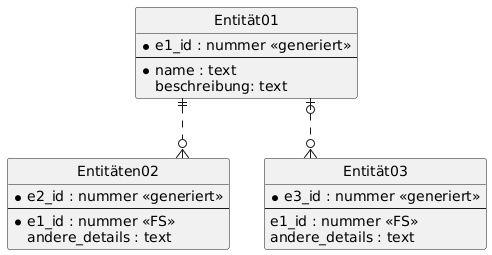
\includegraphics[width=0.81\columnwidth]{graphic2.png}
        \caption{Example figure}
        \label{fig:figure1}
    \end{figure}
        
    Lorem ipsum dolor sit amet, consetetur sadipscing elitr, sed diam nonumy eirmod tempor invidunt ut labore et dolore magna aliquyam erat, sed diam voluptua. At vero eos et accusam et justo duo dolores et ea rebum. Stet clita kasd gubergren, no sea takimata sanctus est Lorem ipsum dolor sit amet. Lorem ipsum dolor sit amet, consetetur sadipscing elitr, sed diam nonumy eirmod tempor invidunt ut labore et dolore magna aliquyam erat, sed diam voluptua. At vero eos et accusam et justo duo dolores et ea rebum. Stet clita kasd gubergren, no sea takimata sanctus est Lorem ipsum dolor sit amet.

    A sample equation \ref{ec:equation}, shows the Schrödinger equation as an example. 
    
        \begin{equation} \label{ec:equation}
            \frac{\hbar^2}{2m}\nabla^2\Psi + V(\mathbf{r})\Psi = -i\hbar \frac{\partial\Psi}{\partial t}
        \end{equation} 
    
    The \textit{amssymb} package was not necessary to include, because stix2 font incorporates mathematical symbols for writing quality equations. In case you choose another font, uncomment the package in \textit{rho class}.

    In case you want to change the values that adjust the spacing above and below in the equations, go to \textit{rho-class/rho.cls/math packages} section and play with \verb|\setlength{\eqskip}{8pt}| value until the preferred spacing is set.

\section{Implementation aspects}

    \subsection{Aspect number 1}

    Lorem ipsum dolor sit amet, consetetur sadipscing elitr, sed diam nonumy eirmod tempor invidunt ut labore et dolore magna aliquyam erat, sed diam voluptua. At vero eos et accusam et justo duo dolores et ea rebum. Stet clita kasd gubergren, no sea takimata sanctus est Lorem ipsum dolor sit amet. Lorem ipsum dolor sit amet, consetetur sadipscing elitr, sed diam nonumy eirmod tempor invidunt ut labore et dolore magna aliquyam erat, sed diam voluptua. At vero eos et accusam et justo duo dolores et ea rebum. Stet clita kasd gubergren, no sea takimata sanctus est Lorem ipsum dolor sit amet.

    Lorem ipsum dolor sit amet, consetetur sadipscing elitr, sed diam nonumy eirmod tempor invidunt ut labore et dolore magna aliquyam erat, sed diam voluptua. At vero eos et accusam et justo duo dolores et ea rebum. Stet clita kasd gubergren, no sea takimata sanctus est Lorem ipsum dolor sit amet. Lorem ipsum dolor sit amet, consetetur sadipscing elitr, sed diam nonumy eirmod tempor invidunt ut labore et dolore magna aliquyam erat, sed diam voluptua. At vero eos et accusam et justo duo dolores et ea rebum. Stet clita kasd gubergren, no sea takimata sanctus est Lorem ipsum dolor sit amet.


    \subsection{Aspect number 2}

\subsection{Inserting Code}

    This class includes the \textit{listings} package, which offers customized features for adding codes specially for C, C++, \LaTeX\ and Matlab. You can customize the format in \textit{rho class} file.


    Lorem ipsum dolor sit amet, consetetur sadipscing elitr, sed diam nonumy eirmod tempor invidunt ut labore et dolore magna aliquyam erat, sed diam voluptua. At vero eos et accusam et justo duo dolores et ea rebum. Stet clita kasd gubergren, no sea takimata sanctus est Lorem ipsum dolor sit amet. Lorem ipsum dolor sit amet, consetetur sadipscing elitr, sed diam nonumy eirmod tempor invidunt ut labore et dolore magna aliquyam erat, sed diam voluptua. At vero eos et accusam et justo duo dolores et ea rebum. Stet clita kasd gubergren, no sea takimata sanctus est Lorem ipsum dolor sit amet.

    Lorem ipsum dolor sit amet, consetetur sadipscing elitr, sed diam nonumy eirmod tempor invidunt ut labore et dolore magna aliquyam erat, sed diam voluptua. At vero eos et accusam et justo duo dolores et ea rebum. Stet clita kasd gubergren, no sea takimata sanctus est Lorem ipsum dolor sit amet. Lorem ipsum dolor sit amet, consetetur sadipscing elitr, sed diam nonumy eirmod tempor invidunt ut labore et dolore magna aliquyam erat, sed diam voluptua. At vero eos et accusam et justo duo dolores et ea rebum. Stet clita kasd gubergren, no sea takimata sanctus est Lorem ipsum dolor sit amet.

    Lorem ipsum dolor sit amet, consetetur sadipscing elitr, sed diam nonumy eirmod tempor invidunt ut labore et dolore magna aliquyam erat, sed diam voluptua. At vero eos et accusam et justo duo dolores et ea rebum. Stet clita kasd gubergren, no sea takimata sanctus est Lorem ipsum dolor sit amet. Lorem ipsum dolor sit amet, consetetur sadipscing elitr, sed diam nonumy eirmod tempor invidunt ut labore et dolore magna aliquyam erat, sed diam voluptua. At vero eos et accusam et justo duo dolores et ea rebum. Stet clita kasd gubergren, no sea takimata sanctus est Lorem ipsum dolor sit amet.
    
    
    \lstinputlisting[caption=Example of matlab code., label={lst:listing-Mat}, language=Matlab]{example.m}

    Insert code with caution. The code must be self explanatory or it must be explained in the text. Only show important parts of your code.
    

Lorem ipsum dolor sit amet, consetetur sadipscing elitr, sed diam nonumy eirmod tempor invidunt ut labore et dolore magna aliquyam erat, sed diam voluptua. At vero eos et accusam et justo duo dolores et ea rebum. Stet clita kasd gubergren, no sea takimata sanctus est Lorem ipsum dolor sit amet. Lorem ipsum dolor sit amet, consetetur sadipscing elitr, sed diam nonumy eirmod tempor invidunt ut labore et dolore magna aliquyam erat, sed diam voluptua. At vero eos et accusam et justo duo dolores et ea rebum. Stet clita kasd gubergren, no sea takimata sanctus est Lorem ipsum dolor sit amet.

\section{Testing}

    Lorem ipsum dolor sit amet, consetetur sadipscing elitr, sed diam nonumy eirmod tempor invidunt ut labore et dolore magna aliquyam erat, sed diam voluptua. At vero eos et accusam et justo duo dolores et ea rebum. Stet clita kasd gubergren, no sea takimata sanctus est Lorem ipsum dolor sit amet. Lorem ipsum dolor sit amet, consetetur sadipscing elitr, sed diam nonumy eirmod tempor invidunt ut labore et dolore magna aliquyam erat, sed diam voluptua. At vero eos et accusam et justo duo dolores et ea rebum. Stet clita kasd gubergren, no sea takimata sanctus est Lorem ipsum dolor sit amet.

    \subsection{Insert a sample figure}


    Lorem ipsum dolor sit amet, consetetur sadipscing elitr, sed diam nonumy eirmod tempor invidunt ut labore et dolore magna aliquyam erat, sed diam voluptua. At vero eos et accusam et justo duo dolores et ea rebum. Stet clita kasd gubergren, no sea takimata sanctus est Lorem ipsum dolor sit amet. Lorem ipsum dolor sit amet, consetetur sadipscing elitr, sed diam nonumy eirmod tempor invidunt ut labore et dolore magna aliquyam erat, sed diam voluptua. At vero eos et accusam et justo duo dolores et ea rebum. Stet clita kasd gubergren, no sea takimata sanctus est Lorem ipsum dolor sit amet.

        Here is how to insert graphics. Upload the file in Overleaf and use the following commands.

        Figure \ref{fig:figure} shows an example figure.
       
        \begin{figure}[H]
            \centering
            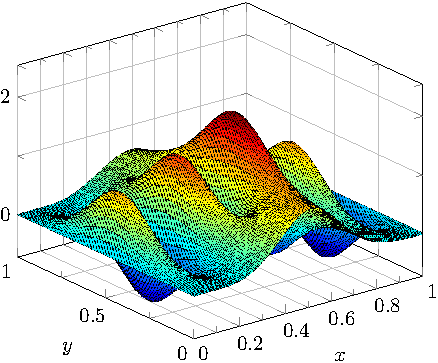
\includegraphics[width=0.71\columnwidth]{Example.pdf}
            \caption{Example figure obtained from PGFPlots \cite{PFGPlots}.}
            \label{fig:figure}
        \end{figure}

    
    \subsection{Sample double figure}

        Figure \ref{fig:examplefloat} shows an example of a two-picture floating figure that covers the width of the page. It can be positioned at the top or bottom of the page. The space between the figures can also be changed using the \verb|\hspace{Xpt}| command.

        \begin{figure*}[t!] % t for position at the top of the current page; b for position at the bottom of the current page
            \centering
                \begin{subfigure}[b]{0.38\linewidth} % Fig (a)
                    \includegraphics[width=\linewidth]{Example2.pdf}
                    \caption{Example left figure.}
                    \label{fig:figa}
                \end{subfigure}
            \hspace{15pt}   % Space between the figures
                \begin{subfigure}[b]{0.38\linewidth} % Fig (b)
                    \centering
                    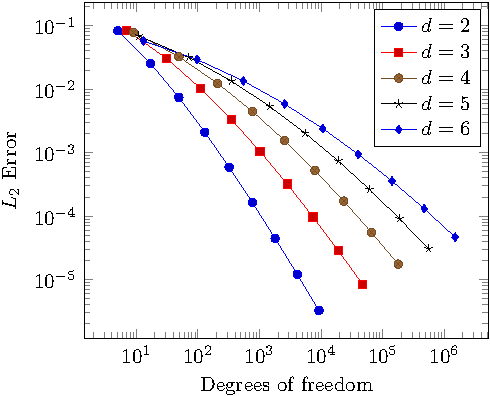
\includegraphics[width=\linewidth]{example2.pdf}
                    \caption{Example right figure.}
                    \label{fig:figb}
                \end{subfigure}
            \caption{Example figure that covers the width of the page obtained from PGFPlots \cite{PFGPlots}.}
            \label{fig:examplefloat}
        \end{figure*}

    Lorem ipsum dolor sit amet, consetetur sadipscing elitr, sed diam nonumy eirmod tempor invidunt ut labore et dolore magna aliquyam erat, sed diam voluptua. At vero eos et accusam et justo duo dolores et ea rebum. Stet clita kasd gubergren, no sea takimata sanctus est Lorem (see \cite{smith2024}, \cite{nasa2024}) ipsum dolor sit amet. Lorem ipsum dolor sit amet, consetetur sadipscing elitr, sed diam nonumy eirmod tempor invidunt ut labore et dolore magna aliquyam erat, sed diam voluptua. At vero eos et accusam et justo duo dolores et ea rebum. Stet clita kasd gubergren, no sea takimata sanctus est Lorem ipsum dolor sit amet.
    
    \subsection{Insert a table}

        In the same way as the figures, you can place tables in one or two columns, depending on the length of the table.

        Table \ref{tab:table}, shows an example table that covers the width of the page positioned at the bottom of a new page.

        \begin{table*}[pb]
            \RaggedRight
            \caption{Table example that covers the width of the page.}
            \label{tab:table}
                \begin{tabular}{lllp{12.2cm}}
                    \toprule
                    \textbf{Day} & \textbf{Min Temp} & \textbf{Max Temp} & \textbf{Summary} \\ 
                    \midrule
                    Monday & 11\textdegree C & 22\textdegree C & A clear day with lots of sunshine.  Strong breeze will bring down the temperatures. \\
                    Tuesday & 9\textdegree C & 19\textdegree C & Cloudy with rain, across many northern regions. \\
                    Wednesday & 10\textdegree C & 21\textdegree C & Rain will still linger for the morning. 
                    Conditions will improve by early afternoon and continue 
                    throughout the evening.\\
                    \bottomrule
                \end{tabular}
                
            \tabletext{Note: Obtained from \LaTeX\ tables \cite{projects-2023}.}
            
        \end{table*}

        Lorem ipsum dolor sit amet, consetetur sadipscing elitr, sed diam nonumy eirmod tempor invidunt ut labore et dolore magna aliquyam erat, sed diam voluptua. At vero eos et accusam et justo duo dolores et ea rebum. Stet clita kasd gubergren, no sea takimata sanctus est Lorem ipsum dolor sit amet. Lorem ipsum dolor sit amet, consetetur sadipscing elitr, sed diam nonumy eirmod tempor invidunt ut labore et dolore magna aliquyam erat, sed diam voluptua. \cite{miller2022} At vero eos et accusam et justo duo dolores et ea rebum. Stet clita kasd gubergren, no sea takimata sanctus est Lorem ipsum dolor sit amet.
    
\section{Summary & Outlook}

    Summarize important information you could gain with the help of these results. Could you finish in time? What should be the next steps?

    Lorem ipsum dolor sit amet, consetetur sadipscing elitr, sed diam nonumy eirmod tempor invidunt ut labore et dolore magna aliquyam erat, sed diam voluptua. At vero eos et accusam et justo duo dolores et ea rebum. Stet clita kasd gubergren, no sea takimata sanctus est Lorem ipsum dolor sit amet. Lorem ipsum dolor sit amet, consetetur sadipscing elitr, sed diam nonumy eirmod tempor invidunt ut labore et dolore magna aliquyam erat, sed diam voluptua. At vero eos et accusam et justo duo dolores et ea rebum. Stet clita kasd gubergren, no sea takimata sanctus est Lorem ipsum dolor sit amet.
    
\section{Appendix}

    You may refer to an external document. Keep in mind to hand in this/these files.
 
%----------------------------------------------------------

% Bibliography is located in a seperate file. Edit the file and add references here in the document. 3-5 Rereferences are sufficiant.

\printbibliography

%----------------------------------------------------------

\end{document}